\subsection{Motivations for Next Generation CSACs}
\label{subsec:motivations}

While current \acrshort{csac} technology offers significant advantages in terms of miniaturization with respect traditional atomic clocks, there is still room for improvement under every aspect of the clock (stability, accuracy, SWaP, etc.).

As it has been with the development of the first \acrshort{csac}, DARPA is again the main driver for the development of \acrshort{ngcsacs}.
Among the funded projects and collaborations with multiple research institutions, three programs are worth to mention:

\begin{itemize}
    \item IMPACT\footnote{Integrated Miniature Primary Atomic Clock Technology (2009-2015).}: aimed to develop a \acrshort{csac} with a volume less than $20cm^3$, a power consumption of $250mW$ and a long-term stability of $\sigma_y(\tau=1month) < 160ns$.
    \item ACES\footnote{Atomic Clock with Enhanced Stability (2015-2022).}: aimed to develop a palm-sized, battery-powered \acrshort{csac} with $1000$ times performance improvement with respect to the current commercial available option.
    \item ROCkN\footnote{Robust Optical Clock Network (2022-ongoing).}: continuation of the ACES program, with the aim of further improving the performances of the clock.
\end{itemize}

The target of these DARPA programs is illustrated in Figure \ref{fig:DARPA-stability-target}.

\begin{figure}[H]
    \centering
    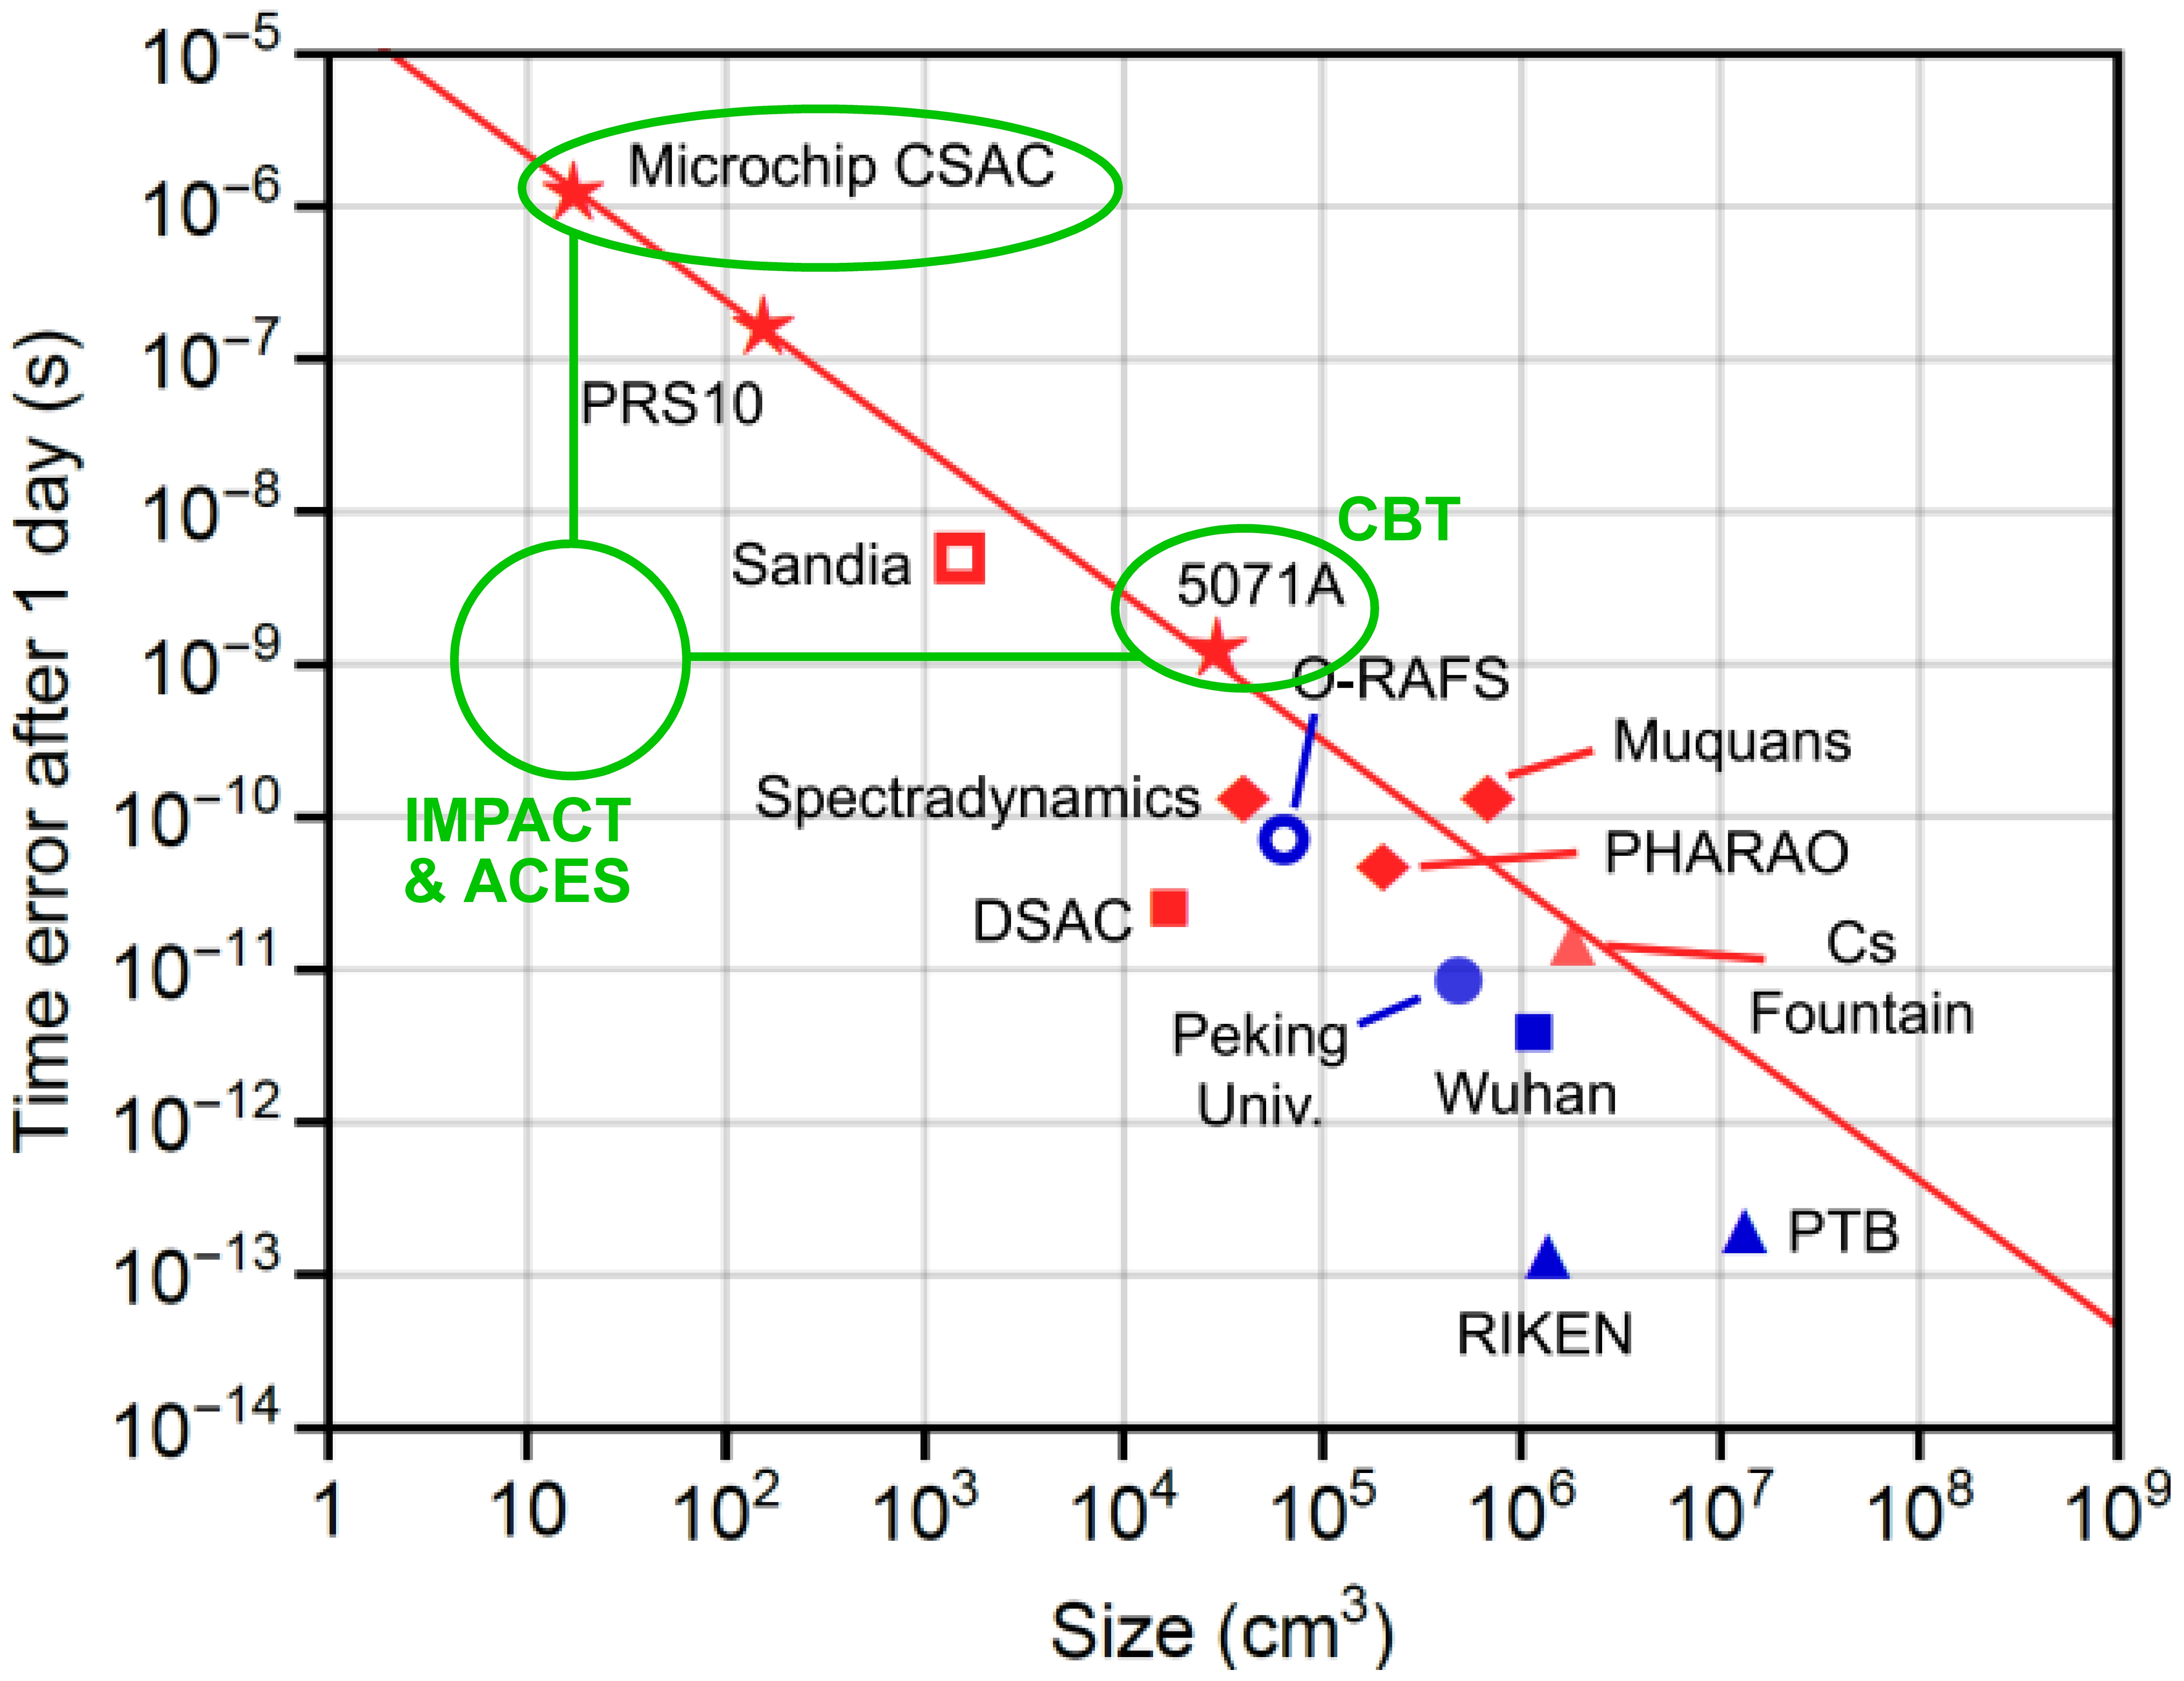
\includegraphics[width=0.6\textwidth, max width=\linewidth]{img/DARPA-stability-target.jpg}
    \caption{Stability vs. Size target for the DARPA IMPACT and ACES programs. Source \cite{Marlow-Scherer}.}
    \label{fig:DARPA-stability-target}
\end{figure}

Generally speaking, \acrshort{ngcsacs} aims to achieve similar quality in terms of performances to the current Cesium Beam Tube (CBT) clock, which is the current standard for high-precision timekeeping, while maintaining the advantages of the \acrshort{csac} technology in terms of size, weight and power consumption.

